\documentclass[11pt]{article}
\usepackage[round,sort&compress]{natbib}
\setcitestyle{aysep={}}
\usepackage{newpxtext,newpxmath}
\usepackage[T1]{fontenc}
\usepackage{hyperref}
\usepackage{graphicx}
\usepackage{amsmath}
\usepackage[left]{lineno}
\linenumbers

\topmargin 0.0cm
\oddsidemargin 0.2cm
\textwidth 16cm
\textheight 21cm
\footskip 1.0cm

\newcommand{\perexpcorrmaps}{S1}
\newcommand{\perexptaskrecon}{S2}
\newcommand{\perexptaskreconseparated}{S3}
\newcommand{\freqpower}{S4}
\newcommand{\networkpower}{S5}
\newcommand{\suppstats}{S6}

% Include your paper's title here

\title{A Gaussian process model of human electrocorticographic data}
\author{
  Lucy L. W. Owen$^{1}$,
  Tudor A. Muntianu$^{1}$,
  Andrew C. Heusser$^{1, 2}$, \\
  Patrick Daly$^{3}$,
  Katherine Scangos$^{3}$, and
  Jeremy R. Manning$^{1\ast}$\\\\
$^{1}$Department of Psychological and Brain Sciences, Dartmouth College,\\
Hanover, NH 03755, USA\\
$^{2}$Akili Interactive,\\
Boston, MA 02110, USA\\
$^{3}$Weill Institute for Neurosciences, University of California, San Francisco,\\
San Francisco, CA 94121, USA}

\date{}

\begin{document}

\baselineskip24pt
\maketitle

\begin{abstract}
  We present a model-based method for inferring full-brain neural
  activity at millimeter-scale spatial resolutions and
  millisecond-scale temporal resolutions using standard human
  intracranial recordings.  Our approach assumes that different
  people's brains exhibit similar correlational structure, and that
  activity and correlation patterns vary smoothly over space.  One can
  then ask, for an arbitrary individual's brain: given recordings from
  a limited set of locations in that individual's brain, along with
  the observed spatial correlations learned from other people's
  recordings, how much can be inferred about ongoing activity at
  \textit{other} locations throughout that
  individual's brain?  We show that our approach generalizes across
  people and tasks, thereby providing a person- and task-general means
  of inferring high spatiotemporal resolution full-brain neural
  dynamics from standard low-density intracranial recordings.
  \\\\
  \footnotesize{\textbf{Keywords: Electrocorticography (ECoG),
      intracranial electroencephalography (iEEG), local field
      potential (LFP), epilepsy, maximum likelihood estimation,
      Gaussian process regression}}
\end{abstract}

\section*{Introduction}
Modern human brain recording techniques are fraught with
compromise~\citep{SejnEtal14}.  Commonly used approaches include
functional magnetic resonance imaging (fMRI), scalp
electroencephalography (EEG), and magnetoencephalography (MEG).  For
each of these techniques, neuroscientists and electrophysiologists
must choose to optimize spatial resolution at the cost of temporal
resolution (e.g., as in fMRI) or temporal resolution at the cost of
spatial resolution (e.g., as in EEG and MEG).  A less widely used
approach (due to requiring work with neurosurgical patients) is to
record from electrodes implanted directly onto the cortical surface
(electrocorticography; ECoG) or into deep brain structures
(intracranial EEG; iEEG).  However, these intracranial approaches also
require compromise: the high spatiotemporal resolution of
intracranial recordings comes at the cost of substantially reduced
brain coverage, since safety considerations limit the number of
electrodes one may implant in a given patient's brain.  Further, the
locations of implanted electrodes are determined by clinical, rather
than research, needs.

An increasingly popular approach is to improve the effective spatial
resolution of MEG or scalp EEG data by using a geometric approach
called \textit{beamforming} to solve the biomagnetic or bioelectrical
inverse problem~\citep{Sarv87}.  This approach entails using detailed
brain conductance models (often informed by high spatial resolution
anatomical MRI images) along with the known sensor placements
(localized precisely in 3D space) to reconstruct brain signals
originating from theoretical point sources deep in the brain (and far
from the sensors).  Traditional beamforming approaches must overcome
two obstacles.  First, the inverse problem beamforming seeks to solve
has infinitely many solutions.  Researchers have made traction towards
constraining the solution space by assuming that signal-generating
sources are localized on a regularly spaced grid spanning the brain
and that individual sources are small relative to their distances to
the sensors~\citep{Snyd91, BailEtal01, HillEtal05}.  The second, and in
some ways much more serious, obstacle is that the magnetic fields
produced by external (noise) sources are substantially stronger than
those produced by the neuronal changes being sought (i.e., at deep
structures, as measured by sensors at the scalp).  This means that
obtaining adequate signal quality often requires averaging the
measured responses over tens to hundreds of responses or trials~\citep[e.g., see review by][]{HillEtal05}.

Another approach to obtaining high spatiotemporal resolution neural data has
been to collect fMRI and EEG data simultaneously. Simultaneous fMRI-EEG has the
potential to balance the high spatial resolution of fMRI with the high temporal
resolution of scalp EEG, thereby, in theory, providing the best of both worlds.
In practice, however, the signal quality of both recordings suffers
substantially when the two techniques are applied simultaneously~\citep[e.g.,
see review by][]{HustEtal12}. In addition, the experimental designs that are
ideally suited to each technique individually are somewhat at odds. For example,
fMRI experiments often lock stimulus presentation events to the regularly spaced
image acquisition time (TR), which maximizes the number of post-stimulus
samples.  By contrast, EEG experiments typically employ jittered stimulus
presentation times to maximize the experimentalist's ability to distinguish
electrical brain activity from external noise sources such as from 60 Hz
alternating current power sources.

The current ``gold standard'' for precisely localizing signals and sampling at
high temporal resolution is to take (ECoG or iEEG) recordings from implanted
electrodes (but from a limited set of locations in any given brain).  This begs
the following question: what can we infer about the activity exhibited by the
rest of a person's brain, given what we learn from the limited intracranial
recordings we have from their brain and additional recordings taken from
\textit{other} people's brains?  Here we develop an approach, which we call
\textit{SuperEEG}\footnote{The term ``SuperEEG'' was coined by Robert J. Sawyer
in his popular science fiction novel \textit{The Terminal
Experiment}~\cite{Sawy95}.  SuperEEG is a fictional technology that measures
ongoing neural activity throughout the entire living human brain with perfect
precision and at arbitrarily high spatiotemporal resolution.}, based on Gaussian
process regression~\citep{Rasm06}.  SuperEEG entails using data from multiple
people to estimate activity patterns at arbitrary locations in each person's
brain (i.e., independent of their electrode placements).  We test our SuperEEG
approach using two large datasets of intracranial recordings~\citep{SedeEtal03,
SedeEtal07a, SedeEtal07b, MannEtal11, MannEtal12, EzzyEtal17, HoraEtal17,
KragEtal17, KuceEtal17, LinEtal17, SoloEtal18, WeidEtal18, EzzyEtal18,
KuceEtal18}.  We show that the SuperEEG algorithm recovers signals well from
electrodes that were held out of the training dataset.  We also examine the
factors that influence how accurately activity may be estimated (recovered),
which may have implications for electrode design and placement in neurosurgical
applications.

\section*{Approach} The SuperEEG approach to inferring high temporal resolution
full-brain activity patterns is outlined and summarized in
Figure~\ref{fig:methods}. We describe (in this section) and evaluate (in
\textit{Results}) our approach using a two large previously collected datasets
comprising multi-session intracranial recordings. Dataset 1 comprises
multi-session recordings taken from 6876 electrodes implanted in the brains of
88 epilepsy patients~\citep{SedeEtal03, SedeEtal07a, SedeEtal07b, MannEtal11,
MannEtal12}.  Each recording session lasted from 0.2--3~h (total recording time:
0.3--14.2~h; Fig.~\suppstats E).  During each recording session, the patients
participated in a free recall list learning task, which lasted for up to
approximately 1~h.  In addition, the recordings included ``buffer'' time (the
length varied by patient) before and after each experimental session, during
which the patients went about their regular hospital activities (confined to
their hospital room, and primarily in bed).  These additional activities
included interactions with medical staff and family, watching television,
reading, and other similar activities.  For the purposes of the Dataset 1
analyses presented here, we aggregated all data across each recording session,
including recordings taken during the main experimental task as well as during
non-experimental time.  We used Dataset 1 to develop our main SuperEEG approach,
and to examine the extent to which SuperEEG might be able to generate
task-general predictions.  Dataset 2 comprised multi-session recordings from
14860 electrodes implanted in the brains of 131 epilepsy
patients~\citep{EzzyEtal17, HoraEtal17, KragEtal17, KuceEtal17, LinEtal17,
SoloEtal18, WeidEtal18, EzzyEtal18, KuceEtal18}.  Each recording session lasted
from 0.4--2.2~h (total recording time: 0.4--6.6~h; Fig.~\suppstats K).  Whereas
Dataset 1 included recordings taken as the patients participated in a variety of
activities, Dataset 2 included recordings taken as each patient performed each
of two specific experimental memory tasks: a random word list free recall task
(Experiment 1) and a categorized word list free recall task (Experiment 2).  We
used Dataset 2 to further examine the ability of SuperEEG to generalize its
predictions within versus across tasks.  Figure~\suppstats~provides additional
information about both datasets.

\begin{figure}
  \centering \includegraphics[width=\textwidth]{figs/methods}
  \caption{\textbf{Methods overview.}  \textbf{A.~Electrode locations.}  Each
  dot reflects the location of a single electrode implanted in the brain of a
  Dataset 1 patient.  A held-out recording location from one patient is
  indicated in red, and the patient's remaining electrodes are indicated in
  black. The electrodes from the remaining patients are colored by $k$-means
  cluster (computed using the full-brain correlation model shown in Panel D).
  \textbf{B.~Radial basis function kernel.} Each electrode contributed by the
  patient (black) weights on the full set of locations under consideration (all
  dots in Panel A, defined as $\bar{R}$ in the text).  The weights fall off with
  positional distance (in MNI space) according to an RBF. \textbf{C.~Per-patient
  correlation matrices.}  After computing the pairwise correlations between the
  recordings from each patient's electrodes, we use RBF-weighted averages to
  estimate correlations between all locations in $\bar{R}$.  We obtain an
  estimated full-brain correlation matrix using each patient's data.
  \textbf{D.~Merged correlation model.}  We combine the per-patient correlation
  matrices (Panel C) to obtain a single full-brain correlation model that
  captures information contributed by every patient.  Here we have sorted the
  rows and columns to reflect $k$-means clustering labels~\citep[using
  $k$=7;][]{YeoEtal11}, whereby we grouped locations based on their correlations
  with the rest of the brain (i.e., rows of the matrix displayed in the panel).
  The boundaries denote the cluster groups.  The rows and columns of Panel C
  have been sorted using the Panel D-derived cluster labels.
  \textbf{E.~Reconstructing activity throughout the brain.}  Given the observed
  recordings from the given patient (shown in black; held-out recording is shown
  in blue), along with a full-brain correlation model (Panel D), we use
  Equation~\ref{eqn:reconstruction} to reconstruct the most probable activity at
  the held-out location (red).} \label{fig:methods}
\end{figure}

We first applied fourth order Butterworth notch filters to remove 60 Hz ($\pm$
.5 Hz) line noise from every recording (from every electrode). Next, we
downsampled the recordings (regardless of the original sample rate) to 250 Hz.
This downsampling step served to both normalize for differences in sampling
rates across patients and to ease the computational burden of our subsequent
analyses.  We then excluded any electrodes that showed putative epileptiform
activity. Specifically, we excluded from further analysis any electrode that
exhibited a maximum kurtosis of 10 or greater across all of that patient's
recording sessions.  We also excluded any patients with fewer than 2 electrodes
that passed this criteria, as the SuperEEG algorithm requires measuring
correlations between 2 or more electrodes from each patient.  For Dataset 1,
this yielded clean recordings from 4168 electrodes implanted throughout the
brains of 67 patients (Fig.~\ref{fig:methods}A, colored dots); for Dataset 2,
this yielded clean recordings from 5023 electrodes implanted in 78 patients.
Each individual patient contributed electrodes from a limited set of brain
locations, which we localized in a common space~\citep[MNI152;][]{GrabEtal06};
an example Dataset 1 patient's 54 electrodes that survived the kurtosis
thresholding procedure are highlighted in black and red
(Fig.~\ref{fig:methods}A).

The recording from a given electrode is maximally informative about the activity
of the neural tissue immediately surrounding its recording surface.  However,
brain regions that are distant from the recording surface of the electrode also
contribute to the recording, albeit (ceteris paribus) to a much lesser extent.
One mechanism underlying these contributions is volume conduction.  The precise
rate of falloff due to volume conduction (i.e., how much a small volume of brain
tissue at location $x$ contributes to the recording from an electrode at
location $\eta$) depends on the size of the recording surface, the electrode's
impedance, and the conductance profile of the volume of brain between $x$ and
$\eta$.  As an approximation of this intuition, we place a Gaussian radial basis
function (RBF) at the location $\eta$ of each electrode's recording surface
(Fig.~\ref{fig:methods}B).  We use the values of the RBF at any brain location
$x$ as a rough estimate of how much structures around $x$ contributed to the
recording from location $\eta$: \begin{align} \mathrm{rbf}(x|\eta,\lambda) & =
\mathrm{exp}\left\{ -\frac{||x - \eta||^2}{\lambda} \right\},\label{eqn:rbf}
\end{align} where the width variable $\lambda$ is a parameter of the algorithm
(which may in principle be set according to location-specific tissue conductance
profiles) that governs the level of spatial smoothing.  In choosing $\lambda$
for the analyses presented here, we sought to maximize spatial resolution (which
implies a small value of $\lambda$) while also maximizing the algorithm's
ability to generalize to any location throughout the brain, including those
without dense electrode coverage (which implies a large value of $\lambda$).
Here we set $\lambda = 20$, guided in part by our prior related
work~\citep{MannEtal14b, MannEtal18}, and in part by examining the brain
coverage with non-zero weights achieved by placing RBFs at each electrode
location in Dataset 1 and taking the sum (across all electrodes) at each voxel
in a 4~mm$^3$ MNI brain.  (We then held $\lambda$ fixed for our analyses of
Dataset 2.)  We note that this value could in theory be further optimized, e.g.,
using cross validation or a formal model~\citep[e.g.,][]{MannEtal18}.

A second mechanism whereby a given region $x$ can contribute to the recording at
$\eta$ is through (direct or indirect) anatomical connections between structures
near $x$ and $\eta$.  Although anatomical and functional correlations can differ
markedly~\citep[e.g.,][]{AdacEtal12, HoneEtal09, GoniEtal14}, we use temporal
correlations in the data to estimate these anatomical
connections~\citep{BeckEtal18}.  Let $\bar{R}$ be the set of locations at which
we wish to estimate local field potentials, and let $R_{s} \subseteq \bar{R}$ be
set of locations at which we observe local field potentials from patient $s$
(excluding the electrodes that did not pass the kurtosis test described above).
In the analyses below we define $\bar{R} = \cup_{s=1}^S R_s$.  We can calculate
the expected inter-electrode correlation matrix for patient $s$, where
$C_{s,k}(i,j)$ is the correlation between the time series of voltages for
electrodes $i$ and $j$ from subject $s$ during session $k$, using:

\begin{align}
  \bar{C}_{s} &=
  \mathrm{r}\left(\frac{1}{n}\left(\sum_{k=1}^{n}\mathrm{z}(C_{s,k})\right)\right),\label{eqn:inter_corr}~\mathrm{where}\\
  \mathrm{z}(r) &= \frac{\log(1+r) - \log(1 - r)}{2}~\mathrm{is~the~Fisher}~z
  \mathrm{-transformation~and}\label{eqn:fishersz}\\ \mathrm{z}^{-1}(z) =
  \mathrm{r}(z) &= \frac{\exp(2z) - 1}{\exp(2z) +
  1}\mathrm{~is~its~inverse}.\label{eqn:invfishersz} \end{align} Next, we use
  Equation~\ref{eqn:rbf} to construct a number of to-be-estimated locations by
  number of patient electrode locations weight matrix, $W_s$.  Specifically,
  $W_s$ approximates how informative the recordings at each location in $R_s$
  are in reconstructing activity at each location in $\bar{R}$, where the
  contributions fall off with an RBF according to the distances between the
  corresponding locations:

\begin{align}
W_s(i, j) = \mathrm{rbf}(i|j,\lambda)\label{eqn:weight_matrix}.
\end{align}

Given this weight matrix, $W_s$, and the observed inter-electrode correlation
matrix for patient $s$, $\bar{C}_{s}$, we can estimate the correlation matrix
for all locations in $\bar{R}$ ($\hat{C}_s$; Fig.~\ref{fig:methods}C) using:

\begin{align}
\hat{N}_{s}(x,y) & = { \sum_{i = 1}^{| R_{s}|}\sum_{j=1}^{i-1} W(x,i) \cdot W(y,j)\cdot \mathrm{z}(\bar{C}_{s}(i,j))}\label{eqn:subj_corrmat_num}\\
 \hat{D}_{s}(x,y) & = \sum_{i = 1}^{| R_{s}|}\sum_{j=1}^{i-1} W(x,i)
                    \cdot W(y,j). \label{eqn:subj_corrmat_den}\\
 \hat{C}_s &= \mathrm{r}\left( \frac{\hat{N}_{s}}{\hat{D}_{s}} \right)
             \label{eqn:subj_corrmat}.
\end{align}
After estimating the numerator ($\hat{N}_{s}$) and denominator
($\hat{D}_{s}$) placeholders for each $\hat{C}_{s}$, we aggregate these
estimates across the $S$ patients to obtain a single expected full-brain
correlation matrix ($\hat{K}$; Fig.~\ref{fig:methods}D):
\begin{align}
 \hat{K} = \mathrm{r} \left(  \frac{\sum_{s=1}^S  \hat{N}_{s}}{\sum_{s=1}^S \hat{D}_{s}}\right).\label{eqn:corrmat}
\end{align}
Intuitively, the numerators capture the general structures of the
patient-specific estimates of full-brain correlations, and the
denominators account for which locations were near the implanted
electrodes in each patient.  To obtain $\hat{K}$, we compute a
weighted average across the estimated patient-specific full-brain
correlation matrices, where patients with observed electrodes near a
particular set of locations in $\hat{K}$ contribute more to the
estimate.

Having used the multi-patient data to estimate a full-brain correlation matrix
at the set of locations in $\bar{R}$ that we wish to know about, we next use
$\hat{K}$ to estimate activity patterns everywhere in $\bar{R}$, given
observations at only a subset of locations in $\bar{R}$
(Fig.~\ref{fig:methods}E).

Let $\alpha_s$ be the set of indices of patient $s$'s electrode locations in
$\bar{R}$ (i.e., the locations in $R_s$), and let $\beta_s$ be the set of
indices of all other locations in $\bar{R}$. In other words, $\beta_s$ reflects
the locations in $\bar{R}$ where we did not observe a recording for patient $s$
(these are the recording locations we will want to fill in using SuperEEG). We
can sub-divide $\hat{K}$ as follows:

\begin{align}
\hat{K}_{\beta_s,\alpha_s} &= \hat{K}(\beta_s,\alpha_s),~\mathrm{and}\label{eqn:Kba}\\
\hat{K}_{\alpha_s,\alpha_s} &= \hat{K}(\alpha_s,\alpha_s)\label{eqn:Kaa}.
\end{align}
Here $\hat{K}_{\beta_s, \alpha_s}$ represents the correlations between
the ``unknown'' activity at the locations indexed by $\beta_s$ and the
observed activity at the locations indexed by $\alpha_s$, and
$\hat{K}_{\alpha_s, \alpha_s}$ represents the correlations between the
observed recordings (at the locations indexed by $\alpha_s$).

Let $Y_{s,k,\alpha_s}$ be the number-of-timepoints ($T$) by
$\left|\alpha_s\right|$ matrix of (observed) voltages from the electrodes in
$\alpha_s$ during session $k$ from patient $s$. Then we can estimate the voltage
from patient $s$'s $k^{th}$ session at the locations in $\beta_s$ as
follows~\citep{Rasm06}:

\begin{align}
\hat{Y}_{s,k,\beta_s} &= ((\hat{K}_{\beta_s,\alpha_s}\cdot\hat{K}_{\alpha_s,\alpha_s}^{-1})\cdot Y_{s,k,\alpha_s}^\mathrm{T})^\mathrm{T}.\label{eqn:reconstruction}
\end{align}
This equation is the foundation of the SuperEEG algorithm.  Whereas we
observe recordings only at the locations indexed by $\alpha_s$,
Equation~\ref{eqn:reconstruction} allows us to estimate the recordings
at all locations indexed by $\beta_s$, which we can define \textit{a priori}
to include any locations we wish, throughout the brain.  This yields
estimates of the time-varying voltages at \textit{every} location in
$\bar{R}$, provided that we define $\bar{R}$ in advance to include the
union of all of the locations in $R_s$ and all of the locations
at which we wish to estimate recordings (i.e., a timeseries of
voltages).

We designed our approach to be agnostic to electrode impedances, as electrodes
that do not exist do not have impedances.  Therefore our algorithm recovers
voltages in standard deviation ($z$-scored) units rather than attempting to
recover absolute voltages. (This property reflects the fact that
$\hat{K}_{\beta_s, \alpha_s}$ and $\hat{K}_{\alpha_s, \alpha_s}$ are correlation
matrices rather than covariance matrices.)  Also, we note that
Equation~\ref{eqn:reconstruction} requires computing a $T$ by $T$ matrix, which
can become computationally intractable when $T$ is very large (e.g., an example
patient in Dataset 1, $T = 51147$; also see Fig.~\suppstats, Panels E and
K). However, because Equation~\ref{eqn:reconstruction} is time invariant, we may
compute $Y_{s,k,\beta_s}$ in a piecewise manner by filling in $Y_{s,k,\beta_s}$
one row at a time (using the corresponding samples from $Y_{s, k, \alpha_s}$).

The SuperEEG algorithm described above and in Figure~\ref{fig:methods} allows us
to estimate, up to a constant scaling factor, local field potentials (LFPs) for
each patient at all arbitrarily chosen locations in the set $\bar{R}$,
\textit{even if we did not record that patient's brain at all of those
locations}.  We next turn to an evaluation of the accuracy of those estimates.

\section*{Results}
We used a cross-validation approach to test the accuracy with
which the SuperEEG algorithm reconstructs activity throughout the brain. For
each patient in turn, we estimated full-brain correlation matrices
(Eqn.~\ref{eqn:corrmat}) using data from all of the \textit{other} patients.
This step ensured that the data we were reconstructing could not also be used to
estimate the between-location correlations that drove the reconstructions via
Equation~\ref{eqn:reconstruction} (otherwise the analysis would be circular).
For that held-out patient, we held out each electrode in turn.  We used
Equation~\ref{eqn:reconstruction} to reconstruct activity at the held-out
electrode location, using the correlation matrix learned from all other
patients' data as $\hat{K}$, and using activity recorded from the other
electrodes from the held-out patient as $Y_{s, k, \alpha_s}$.  We then asked:
how closely did each of the SuperEEG-estimated recordings at those electrodes
match the observed recordings from those electrodes (i.e., how closely did the
estimated $\hat{Y}_{s, k, \beta_s}$ match the observed $Y_{s, k, \beta_s}$)?

We used this general approach to quantify the algorithm's performance across the
full dataset. For each held-out electrode, from each held-out patient in turn,
we computed the average correlation (across recording sessions) between the
SuperEEG-reconstructed voltage traces and the observed voltage traces from that
electrode.  For this analysis we set $\bar{R}$ to be the union of all electrode
locations across all patients.  This yielded a single correlation coefficient
for each electrode location in $\bar{R}$, reflecting how well the SuperEEG
algorithm was able to recover the recording at that location by incorporating
data across patients (black histogram in Fig.~\ref{fig:corrmap}A, map in
Fig.~\ref{fig:corrmap}C).  The observed distribution of correlations was
centered well above zero (mean: 0.51; $t$-test comparing mean of distribution of
$z$-transformed average patient correlation coefficients to 0: $t(66) = 23.55, p
< 10^{-10}$), indicating that the SuperEEG algorithm recovers held-out activity
patterns substantially better than random guessing.

Next, we compared the quality of these across-participant reconstructions (i.e.,
computed using a correlation model learned from other patients' data) to
reconstructions generated using a correlation model trained using the
in-patient's data.  In other words, for this within-patient benchmark analysis
we estimated $\hat{C}_{s}$ (Eqn.~\ref{eqn:subj_corrmat}) for each patient in
turn, using recordings from all of that patient's electrodes except at the
location we were reconstructing.  These within-patient reconstructions serve as
an estimate of how well data from all of the other electrodes from that single
patient may be used to estimate held-out data from the same patient.  This
allows us to ask how much information about the activity at a given electrode
might be inferred through (a) volume conductance or other sources of ``leakage''
from activity patterns measured from the patient's other electrodes and (b)
across-electrode correlations learned from that single patient.  As shown in
Figure~\ref{fig:corrmap}A (gray histogram), the distribution of within-patient
correlations was centered well above zero (mean: 0.32; $t$-test comparing mean
of distribution of $z$-transformed average patient correlation coefficients to
0: $t(66) = 15.16, p < 10^{-10}$). However, the across-patient correlations were
substantially higher ($t$-test comparing average $z$-transformed within versus
across patient electrode correlations: $t(66) = 9.17, p < 10^{-10}$).  This is
an especially conservative test, given that the across-patient SuperEEG
reconstructions exclude (from the correlation matrix estimates) all data from
the patient whose data is being reconstructed.  We repeated each of these
analyses on a second independent dataset and found similar results
(Fig.~\ref{fig:corrmap}B, D; within versus across reconstruction accuracy:
$t(77) = 11.25, p < 10^{-10}$). We also replicated this result separately for
each of the two experiments from Dataset 2 (Fig.~\perexpcorrmaps).  This overall
finding, that reconstructions of held-out data using correlation models learned
from \textit{other} patient's data yield higher reconstruction accuracy than
correlation models learned from the patient whose data is being reconstructed,
has two important implications.  First, it implies that distant electrodes
provide additional predictive power to the data reconstructions beyond the
information contained solely in nearby electrodes.  (This follows from the fact
that each patient's grid, strip, and depth electrodes are implanted in a unique
set of locations, so for any given electrode the closest electrodes in the full
dataset tend to come from the same patient.)  Second, it implies that the
spatial correlations learned using the SuperEEG algorithm are, to some extent,
similar across people.

%correlations by brain area, distribution of correlations
\begin{figure}
  \centering 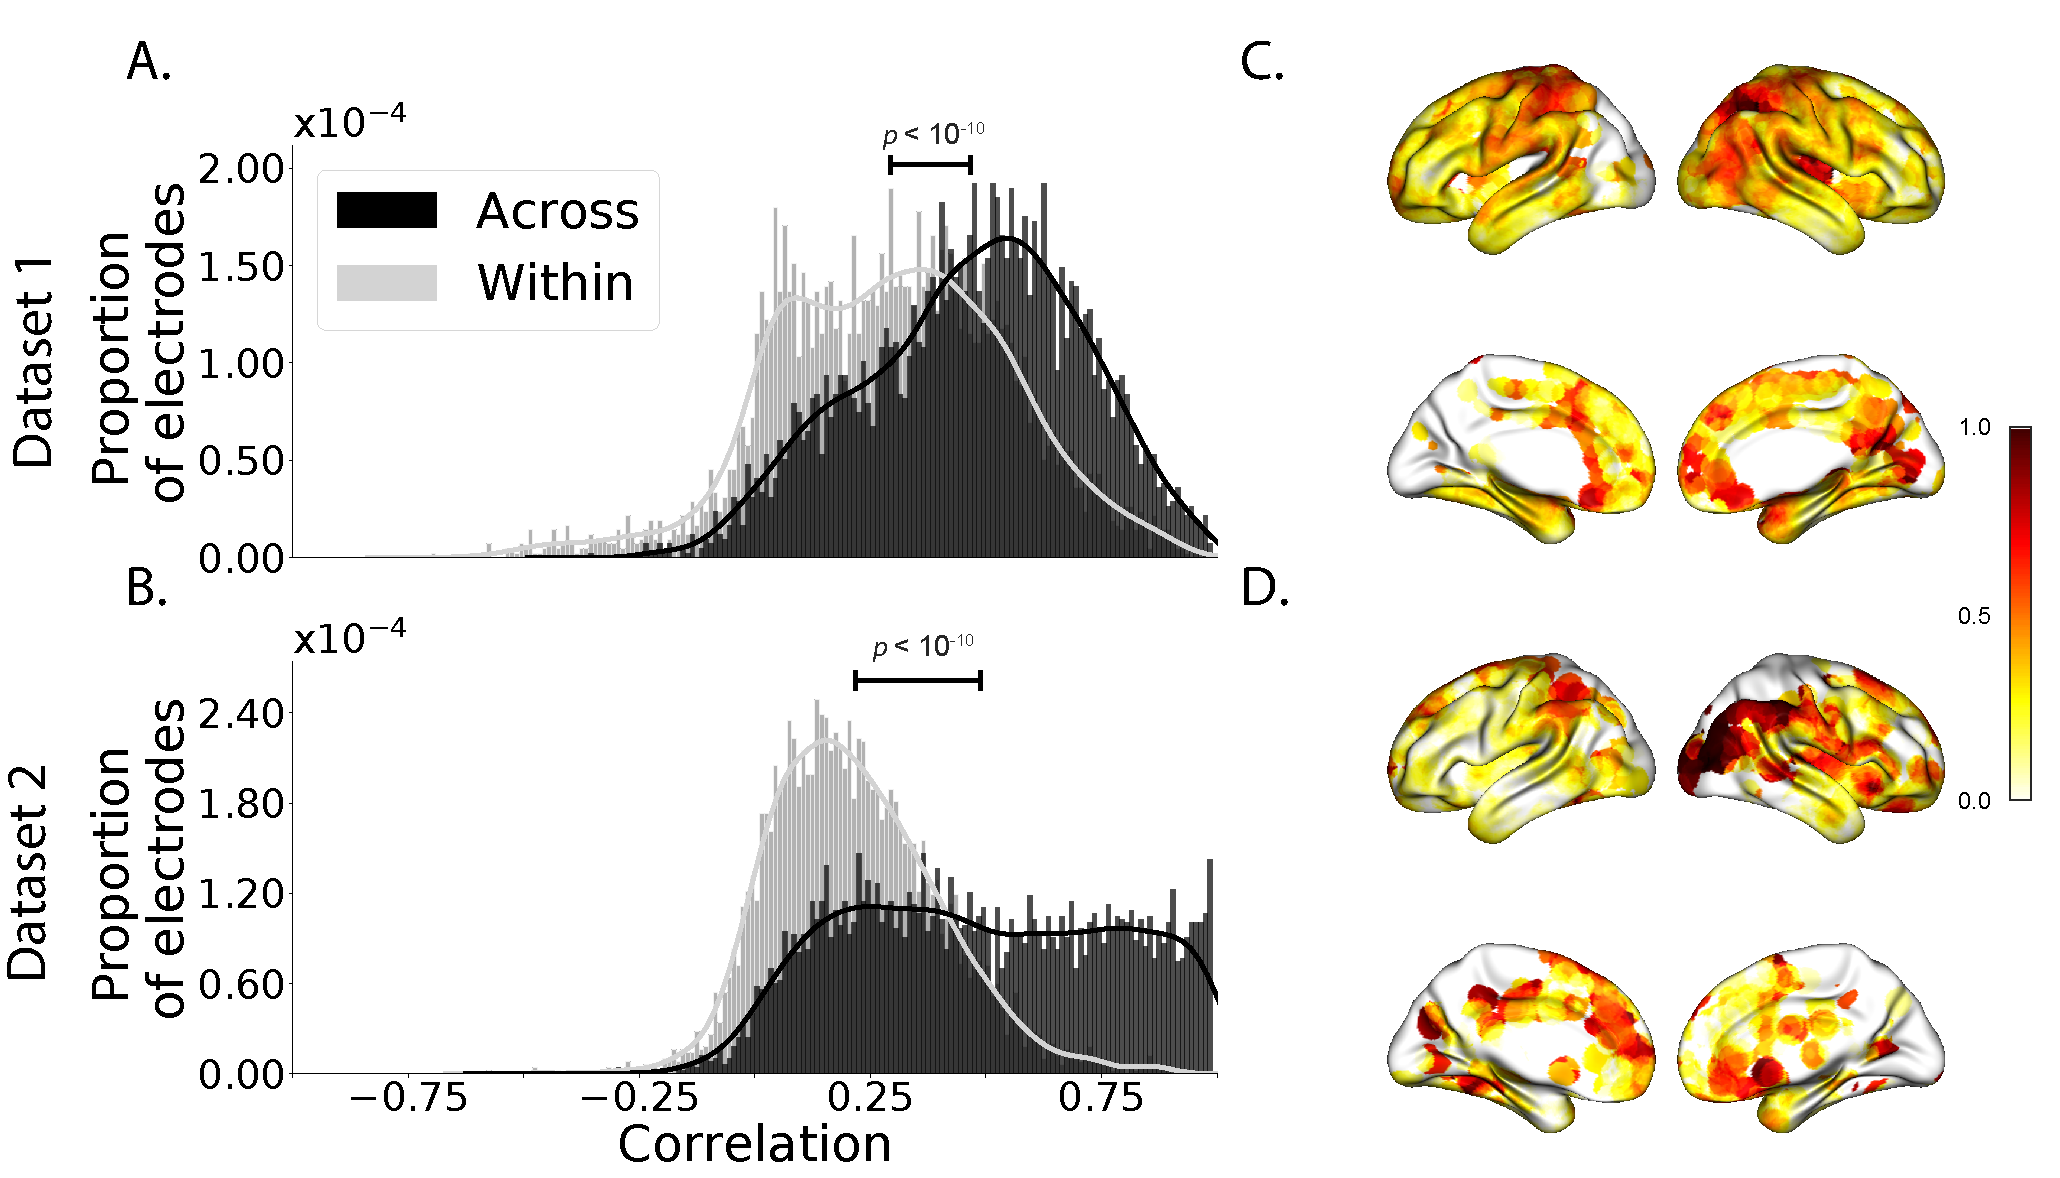
\includegraphics[width=\textwidth]{figs/corrmap}
  \caption{\textbf{Reconstruction accuracy across all electrodes in two ECoG
  datasets.}  \textbf{A. Distributions of correlations between observed versus
  reconstructed activity by electrode, for Dataset 1.}  The across-patient
  distribution (black) reflects reconstruction accuracy (correlation) using a
  correlation model learned from all but one patient's data, and then applied to
  that held-out patient's data.  The within-patient distribution (gray) reflects
  performance using a correlation model learned from the same patient who
  contributed the to-be-reconstructed electrode. \textbf{B. Distributions of
  correlations for Dataset 2.}  This panel is in the same format as Panel A, but
  reflects results obtained from Dataset 2.  The histograms aggregate data
  across both Dataset 2 experiments; for results broken down by experiment see
  Figure~\perexptaskreconseparated. \textbf{C.--D.  Reconstruction accuracy by
  location.} The colors denote the average across-session correlations, using
  the across-patient correlation model, between the observed and reconstructed
  activity at the given electrode location projected to the cortical
  surface~\citep{CombEtal19}.  Panel C displays the map for Dataset 1 and Panel
  D displays the map for Dataset 2.} \label{fig:corrmap}
\end{figure}

The recordings we analyzed from Dataset 1 comprised data collected as the
patients performed a variety of (largely idiosyncratic) tasks throughout each
day's recording session.  That we observed reliable reconstruction accuracy
across patients suggests that the spatial correlations derived from the SuperEEG
algorithm are, to some extent, similar across tasks.  We tested this finding
more directly using Dataset 2.  In Dataset 2, the recordings were limited to
times when each patient was participating in one of two experiments.  Experiment
1 is a random-word list free recall task; Experiment 2 is a categorized list
free recall task (24 patients particpated in both).  We wondered whether a
correlation model learned from data from one experiment might yield good
predictions of data from the other experiment.  Further, we wondered about the
extent to which it might be beneficial or harmful to combine data across tasks.

To test the task-specificity of the SuperEEG-derived correlation models, we
restricted the dataset to the 24 patients that participated in both experiments
and repeated the above within- and across-patient cross validation procedures
separately for Experiment 1 and Experiment 2 data from Dataset 2.  We then
compared the reconstruction accuracies for held-out electrodes, for models
trained within versus across the two experiments, or combining across both
experiments (Fig.~\perexptaskrecon).  In every case we found that across-patient
models trained using data from all other patients out-performed within-patient
models trained on data only from the subject contributing the given electrode
($t$s$(23) > 6.50, p$s$ < 10^{-5}$). All reconstruction accuracies also reliably
exceeded chance performance ($t$s$(23) > 8.00, p$s$ < 10^{-8}$).  Average
reconstruction accuracy was highest for the across-patient models limited to
data from the same experiment (mean accuracy: $0.68$); next-highest for the
models that combined data across both experiments (mean accuracy: $0.61$); and
lowest for models trained across tasks (mean accuracy: $0.47$).  This pattern of
results also held for each of the Dataset 2 experiments individually
(Fig.~\perexptaskreconseparated).  Taken together, these results indicate that
there are reliable commonalities in the spatial correlations of full-brain
activity across tasks, but that there are also reliable differences in these
spatial correlations across tasks. Whereas reconstruction accuracy benefits from
incorporating data from other patients, reconstruction accuracy is highest when
constrained to within-task data, or data that includes a variety of tasks (e.g.,
Dataset 1, or combining across the two Dataset 2 experiments).

Although both datasets we examined provide good full-brain coverage (when
considering data from every patient), electrodes were not sampled uniformly
throughout the brain.  For example, electrodes are more likely to be implanted
in regions like the medial temporal lobe (MTL), and are rarely implanted in
occipital cortex (Fig.~\ref{fig:density}A, B). Separately for each dataset, for
each voxel in the 4~mm$^3$ voxel MNI152 brain, we computed the proportion of
electrodes in the dataset that were contained within a 20 MNI unit radius sphere
centered on that voxel.  We defined the \textit{density} at that location as
this proportion. Across Datasets 1 and 2, the electrode placement densities were
similar (correlation by voxel: $r = 0.6, p < 10^{-10}$).  We wondered whether
regions with good covererage might be associated with better reconstruction
accuracy. For example, Figures~\ref{fig:density}A and B indicate that many
electrodes in the MTL (which tends to be relatively densely sampled) have
relatively high reconstruction accuracy, and occipital electrodes (which tends
to be relatively sparsely sampled) tend to have relatively low reconstruction
accuracy.  To test whether this held more generally across the entire brain, for
each dataset we computed the electrode placement density for each electrode from
each patient (using the proportion of \textit{other} patients' electrodes within
20 MNI units of the given electrode).  We then correlated these density values
with the across-patient reconstruction accuracies for each electrode.  We found
no reliable correlation between reconstruction accuracy and density for Dataset
1 ($r = 0.05, p = 0.70$) and a reliable negative correlation for Dataset 2 ($r =
-0.21, p = 0.05$).  This indicates that the reconstruction accuracies we
observed are \textit{not} driven solely by sampling density, but rather may also
reflect higher order properties of neural dynamics such as functional
correlations between distant voxels~\citep{BetzEtal17b}.

Prior work in humans and animals has shown that the spatial profile of the local
field potential differs by frequency band~\citep[e.g., with respect to volume
conductance properties and contribution to the local field
potential;][]{BuzsEtal12, FrieEtal07, CronEtal11}.  For example, lower frequency
components of the local field potential tend to have higher power and extend
further in space than high-frequency components~\citep[e.g., ][]{MillEtal07,
MannEtal09}.  We therefore wondered whether the reconstructions we observed
might be differently weighting or considering the contributions of activity at
different frequency bands.  We therefore examined a range of frequency bands
($\delta$: 2--4 Hz; $\theta$: 4--8 Hz; $\alpha$: 8--12 Hz; $\beta$: 12--30 Hz;
$\gamma_L$: 30--60 Hz; and $\gamma_H$: 60--100 Hz), along with a measure of
broadband power.  We defined broadband power as the mean height of a linear
robust regression fit in log-log space to the order 4 Morelet wavelet-computed
power spectrum at 50 log-spaced frequencies from from 2--100
Hz~\citep{MannEtal09}. We used second-order Butterworth bandpass filters to
compute the activity patterns within each narrow frequency band.  We then
repeated our within-subject and across-subject cross-validated reconstruction
accuracy tests (analogous to Fig.~\ref{fig:corrmap}) separately for each
frequency band (Fig.~\ref{fig:frequency}).  (We also carried out a similar
analysis on the Hilbert transform-computed spectral power within each narrow
band; see Fig.~\freqpower.)  Across both datasets, we found that our approach is
best at reconstructing patterns of broadband activity (right-most bars in
Figs.~\ref{fig:frequency}A and D), a correlate of population firing
rate~\citep{MannEtal09}.  We also achieved good reconstruction accuracy within
each narrow frequency band (Figs.~\ref{fig:frequency} and \freqpower).  Activity
at lower frequencies ($\delta$, $\theta$, $\alpha$, and $\beta$) tended to be
reconstructed better than high-frequency patterns ($\gamma_L$ and $\gamma_H$),
with reconstruction accuracy peaking in the $\alpha$ band.  Overall, these
results indicate that our approach is able to accurately recover information
within the 2--100 Hz range, although those reconstructions are most accurate for
low-frequency or broadband patterns.

\begin{figure}
  \centering 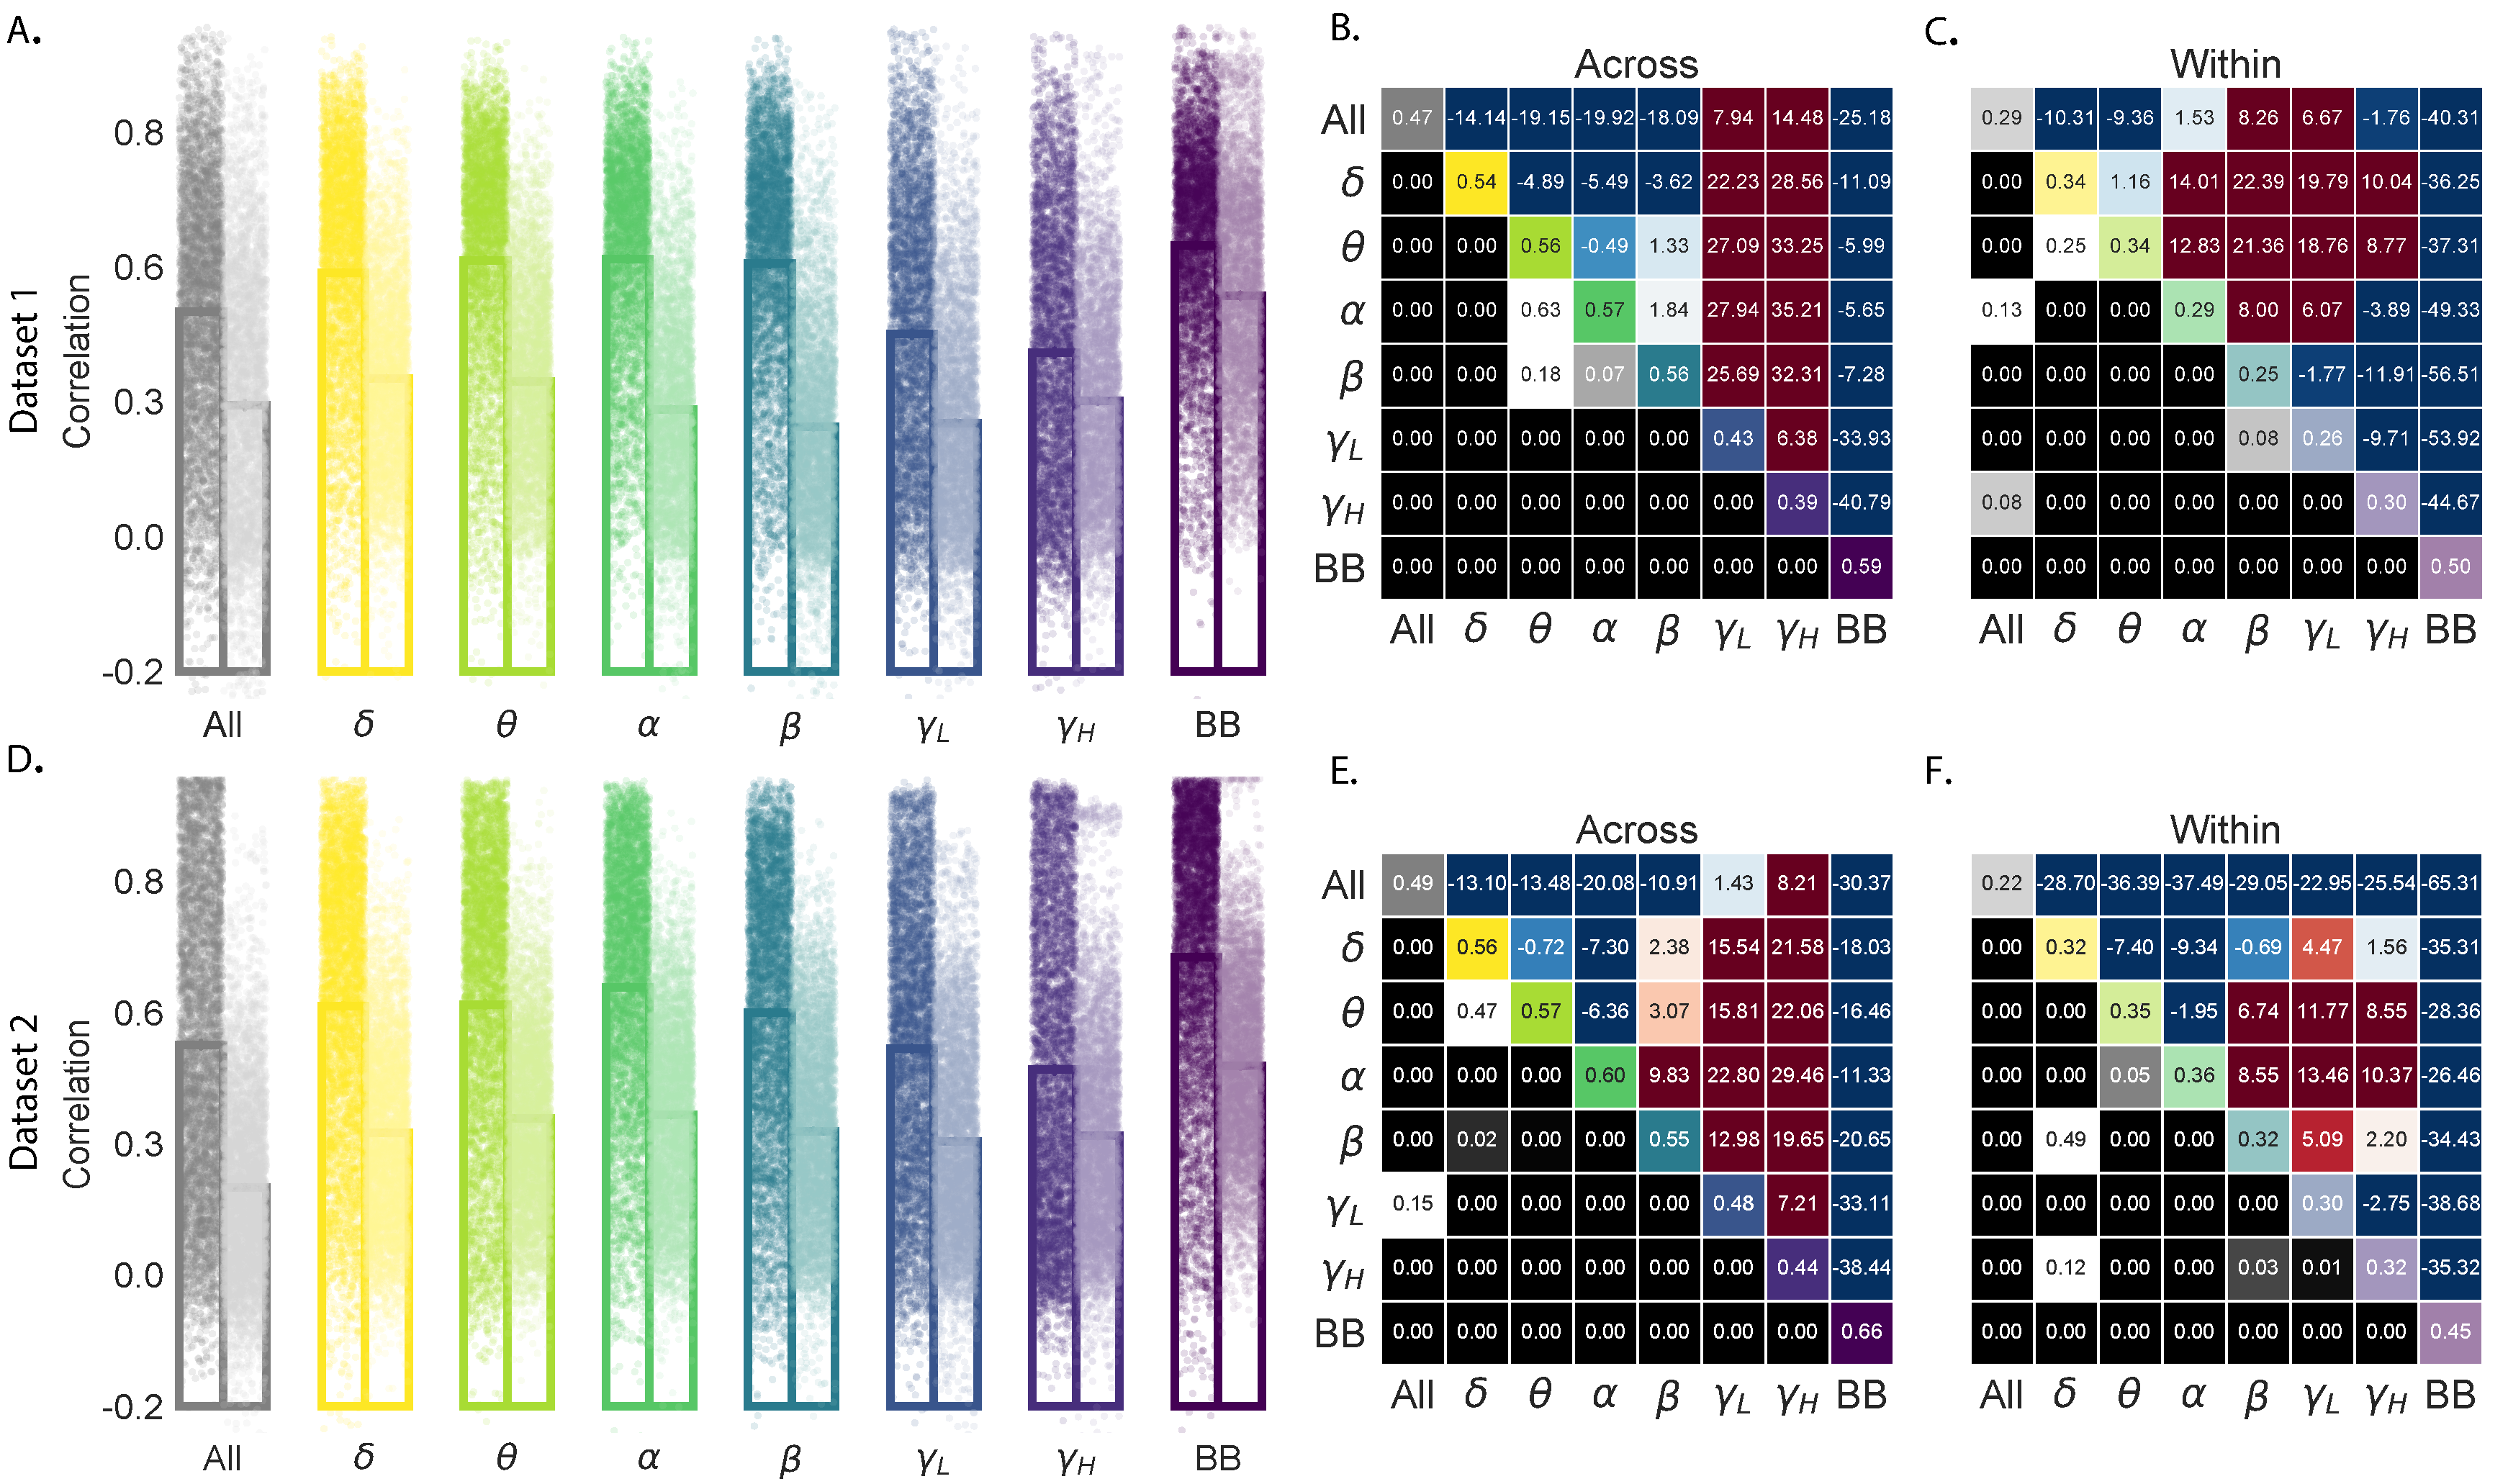
\includegraphics[width=\textwidth]{figs/frequency}
  \caption{\textbf{Reconstruction accuracy across all electrodes in two ECoG
  datasets for each frequency triangles.} \textbf{A. Distributions of
  correlations between observed versus reconstructed activity by electrode, for
  each frequency band in Dataset 1.}  Each color denotes a different frequency
  range. Within each color group, the darker dots and bar on the left display
  the distribution (and mean) across-patient reconstruction accuracies
  (analogous to the black histograms in Fig.~\ref{fig:corrmap}).  The lighter
  dots and bar on the right display the distribution (and mean) within-patient
  reconstruction accuracies (analogous to the gray histograms in
  Fig.~\ref{fig:corrmap}). To facilitate visual comparison with the
  frequency-specific results, the leftmost bars (gray) re-plot the histograms in
  Fig.~\ref{fig:corrmap}A. \textbf{B.~Statistical summary of across-patient
  reconstruction accuracy by electrode for each frequency band in Dataset 1.} In
  the upper triangles of each map, warmer colors (positive $t$-values) indicate
  that the distribution of reconstruction accuracy for the frequency band in a
  given row yielded was greater than the frequency band in the given column.
  Cooler colors (negative $t$-values) indicate that the frequency band in the
  given row yielded lower reconstruction accuracy than the frequency band in the
  given column. The lower triangles of each map denote the corresponding
  $p$-values for the $t$-tests. The diagonal entries display the average
  reconstruction accuracy within each frequency band. \textbf{C.~Statistical
  summary of within-patient reconstruction accuracy by electrode for each
  frequency band in Dataset 1.} This panel displays the within-patient
  statistical summary, in the same format as Panel B.  \textbf{D.~Distributions
  of correlations between observed versus reconstructed activity by electrode,
  for each frequency band in Dataset 2.}  This panel displays reconstruction
  accuracy distributions for each frequency range for Dataset 2.
  \textbf{E.--F.~Statistical summaries of across-patient and within-patient
  reconstruction accuracy by electrode for each frequency band in Dataset 2.}
  These panels are in the same as Panels B and C, but display results from
  Dataset 2.} \label{fig:frequency}
\end{figure}


\begin{figure}
  \centering 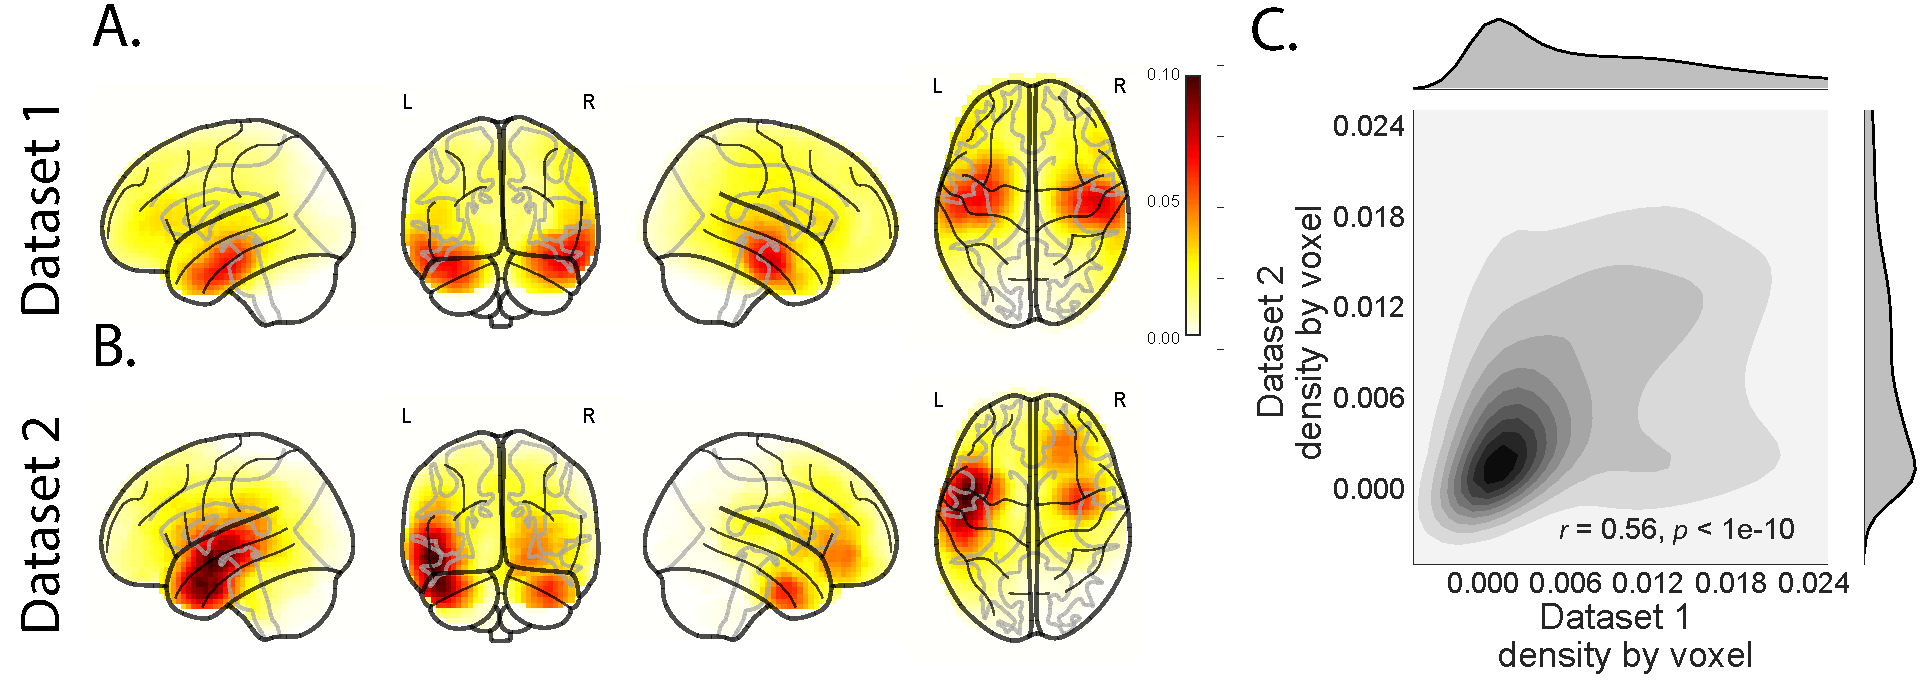
\includegraphics[width=\textwidth]{figs/density}
  \caption{\textbf{Electrode sampling density by location.} \textbf{A.~Electrode
  sampling density by voxel location in Dataset 1.} Each voxel is colored by the
  proportion of total electrodes in the dataset that are located within a 20~MNI
  unit radius sphere centered on the given voxel.  \textbf{B.~Electrode sampling
  density by voxel location in Dataset 2.}  This panel displays the sampling
  density map for Dataset 2, in the same format as Panel A.
  \textbf{C.~Correspondence in sampling density by voxel location across
  Datasets 1 and 2.}  The two-dimensional histogram displays the per-voxel
  sampling densities in the two Datasets, and the one-dimensional histograms
  display the proportions of voxels in each dataset with the given density
  value.  The correlation reported in the panel is across voxels in the 4~mm$^3$
  MNI152 brain.} \label{fig:density}
\end{figure}

A basic assumption of our approach (and of most prior ECoG work) is that
electrode recordings are most informative about the neural activity near the
recording surface of the electrode.  But if we consider that activity patterns
throughout the brain are meaningfully correlated, are there particular
implantation locations that, recorded from in a given patient's brain, yield
especially high reconstruction accuracies throughout the rest of their brain?
For example, one might hypothesize that brain structures that are heavily
interconnected with many other structures could be more informative about
full-brain activity patterns than comparatively isolated structures.  To test
this hypothesis, we computed the average reconstruction accuracy across all of
each patient's electrodes (using our across-patients cross validation test;
black histograms in Fig.~\ref{fig:corrmap}A and B).  We first labeled each
patient's electrodes, in each dataset, with the average reconstruction accuracy
for that patient.  In other words, we assigned every electrode from each patient
the same value, reflecting how well the activity patterns for that patient were
reconstructed. Next, for each voxel in the 4~mm$^3$ MNI brain, we computed the
average value across any electrode (from any patient) that came within 20 MNI
units of that voxel's center.  This yielded an \textit{information score} for
each voxel, reflecting the average reconstruction accuracy across any patients
with electrodes near each voxel-- where the averages were weighted to reflect
patients who had more electrodes implanted near that location. We created a
single map of these information scores for each dataset, highlighting regions
that are especially informative about activity in \textit{other} brain areas
(Fig.~\ref{fig:informap}A and B).  Despite task and patient differences across
the two datasets, we nonetheless found that the maps of the most promising
implantation targets derived from both datasets were correlated (voxel-wise
correlation between information scores across the two datasets: $r = 0.18, p <
10^{-10}$).  Our finding that there were some commonalities between the two
datasets' maps lends support to the notion that different brain areas are
(reliably) differently informative about full-brain activity patterns.  We also
examined the intersection between the top 10\% most informative voxels across
the two datasets (gray areas in Fig.~\ref{fig:informap}C, networks shown in
Fig.~\ref{fig:networks}A, top row). Supporting the notion that structures that
are highly interconnected with the rest of the brain are most informative about
full-brain activity patterns, the intersecting set of voxels with the highest
information scores included major portions of the dorsal attention network
(e.g., inferior parietal lobule, precuneus, inferior temporal gyrus, thalamus,
and striatum) as well as some portions of the default mode network (e.g.,
angular gyrus) that are highly interconnected with a large proportion of the
brain's gray matter~\citep[e.g.,][]{TomaVolk11}.

\begin{figure}
  \centering 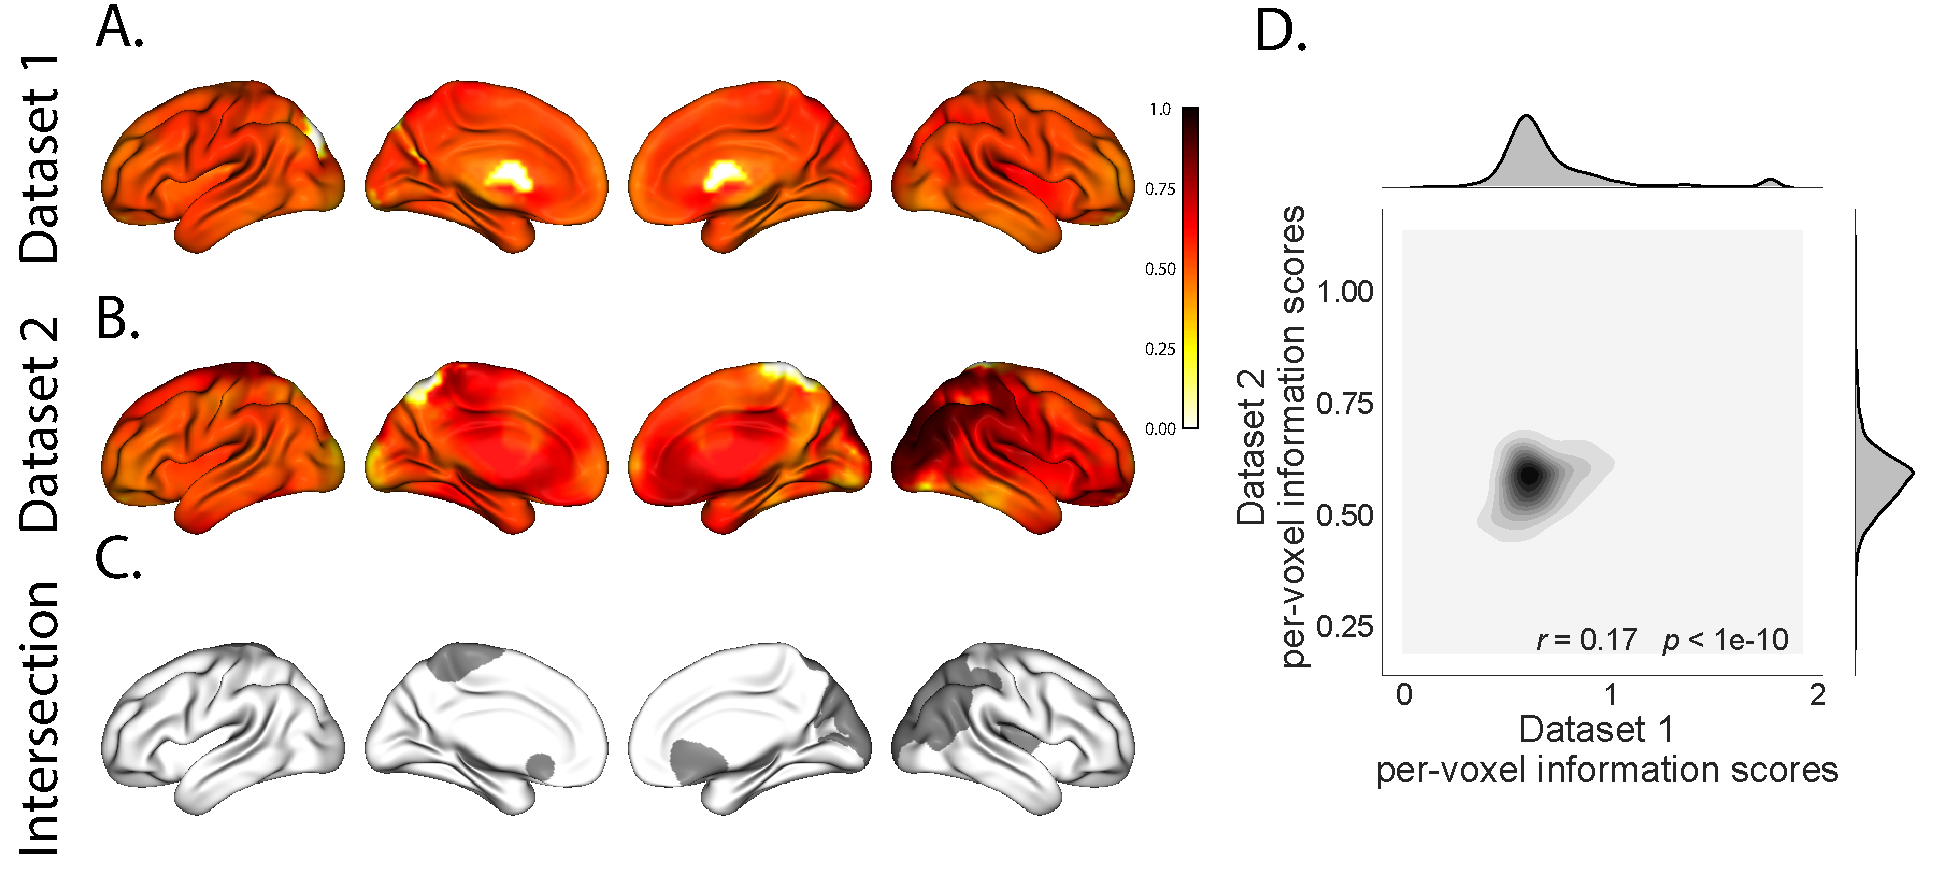
\includegraphics[width=\textwidth]{figs/informap}
  \caption{\textbf{Most informative recording locations.} \textbf{A. Dataset 1
  information scores by voxel.} The voxel colors reflect the weighted average
  reconstruction accuracy across all electrodes from any patients with at least
  one electrode within 20 MNI units of the given voxel.  \textbf{B. Dataset 2
  information scores by voxel.}  This panel is in the same format as Panel A.
  \textbf{C. Intersection.} Gray areas indicate the intersections between the
  top 10\% most informative voxels in each map and projected onto the cortical
  surface~\citep{CombEtal19}. \textbf{D. Correspondence in information scores by
  voxel across Datasets 1 and 2.}  The correlation reported in the Panel is
  between the per-voxel information scores across Datasets 1 and 2.}
  \label{fig:informap}
\end{figure}

We also wondered whether the map of information scores might vary as a function
of the spectral components of the activity patterns under consideration.  We
computed analogous maps of information scores for each individual frequency
range. Across Datasets 1 and 2 (with the exception of $\alpha$ band activity),
we observed reliable positive correlations between the voxel-by-voxel maps of
information scores ($\delta$: $r = 0.09, p < 10^{-57}$; $\theta$: $r = 0.24, p <
10^{-60}$; $\alpha$: $r = -0.03, p < 0.001$, $\beta$: $r = 0.02, p - 0.0011$;
$\gamma_L$: $r = 0.1, p < 10^{-67}$; $\gamma_H$: $r = 0.03, p < 10^{-7}$;
broadband: $r = 0.21, p < 10^{-297})$.

To gain additional insight into which regions were most informative about
full-brain activity patterns at different frequency ranges, we next computed
(for each frequency range) the intersection of the top 10\% highest information
scores across the maps for Datasets 1 and 2 (analogous to our approach in
Fig.~\ref{fig:informap}C). This yielded a single map of the (reliably) most
informative locations, for each frequency range we examined. We then carried out
\textit{post hoc} analyses on each of these maps to better characterize the
underlying structural and functional properties of each set of regions we
identified as being particularly informative about one or more neural patterns.

A growing body of neuroscientific research is concerned with characterizing the
\textit{parcellations} of anatomical and functional brain networks~\citep[for
review see][]{ZaleEtal10, ArslEtal18}. The dominant approaches entail obtaining
a full-brain connectivity matrix using either diffusion tensor imaging to
identify the brain's network of white matter connections, or functional
connectivity (typically applied to resting state data) to correlate the patterns
of activity exhibited by different brain structures.  One can then apply graph
theoretic approaches to assign each brain structure (typically a single fMRI
voxel) to one or more networks~\citep[for review see][]{BullSpor09}. The result
is a set of distinct (or partially overlapping) brain ``networks'' that may be
further examined to elucidate their potential functional role.  We overlaid a
well-cited seven-network parcellation map identified by \cite{YeoEtal11} onto
the maps of brain locations that were most informative about each type of neural
pattern.  For each of these information maps, we computed the proportion of
voxels in the most informative brain regions that belonged to each of the seven
networks identified by \cite{YeoEtal11}; Figure~\ref{fig:networks}D. We found
that the regions we identified as being most informative about different neural
patterns varied markedly with respect to which functional networks they belonged
to (Fig.~\ref{fig:networks}A, B).

\begin{figure}
  \centering 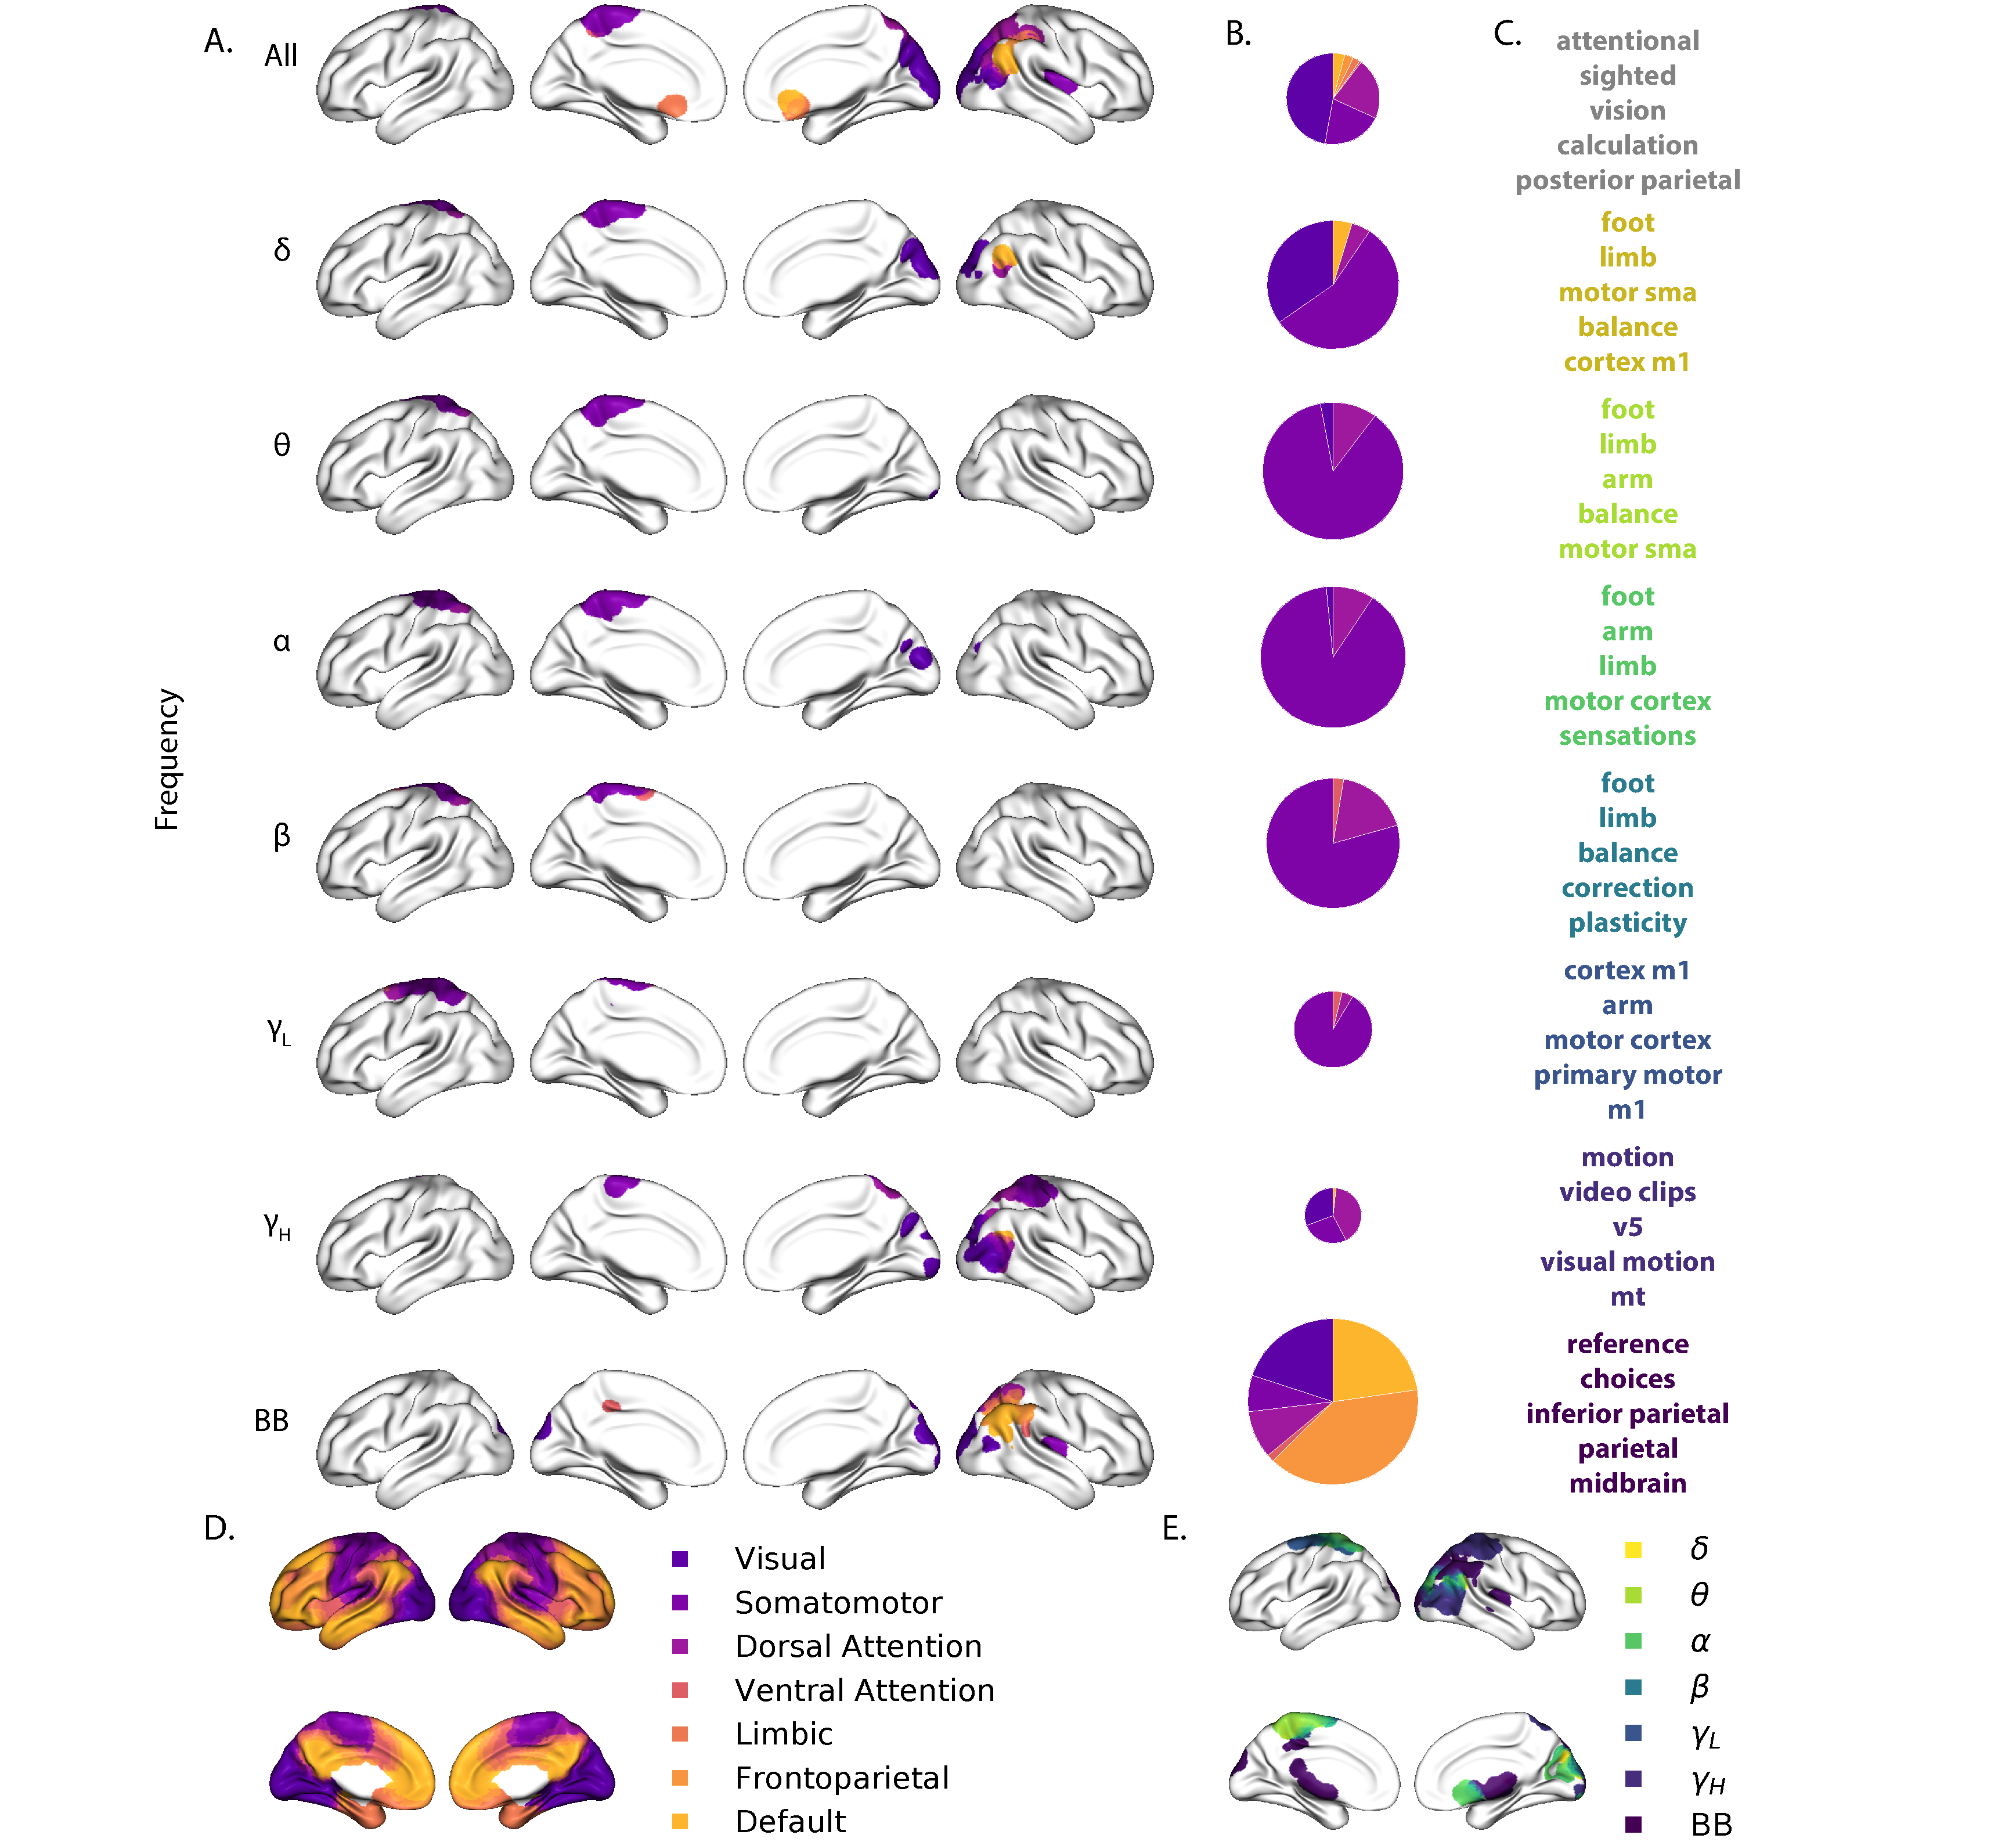
\includegraphics[width=\textwidth]{figs/networks}
  \caption{\textbf{Most informative recording locations by frequency range.}
  \textbf{A.~Intersections between information score maps by frequency range.}
  The regions indicated in each row depict the intersection between the top 10\%
  most informative locations across Datasets 1 and 2.  \textbf{B.~Network
  memberships of the most informative brain regions.}  The pie charts display
  the proportions of voxels in each region that belong to the seven networks
  identified by \cite{YeoEtal11}.  The relative sizes of the charts for each
  frequency range reflct the average across-subject reconstruction accuracies
  (Fig.~\ref{fig:corrmap}A, D).  The voxels in Panel A are colored according to
  the same network memberships.  \textbf{C.~Neurosynth terms associated with the
  most informative brain regions, by frequency range.}  The lists in each row
  display the top five neurosynth terms~\citep{RubiEtal17} decoded for each
  region.  \textbf{D.~Network parcellation map and legend.}  The parcellation
  defined by \cite{YeoEtal11} is displayed on the inflated brain maps.  The
  colors and network labels serve as a legend for Panels A and B.
  \textbf{E.~Combined map of the most informative brain regions.}  The map
  displays the union of the most informative maps in Panel A, colored by
  frequency range.  The labels also serve as a legend for Panel C.}
  \label{fig:networks}
\end{figure}

The frequency-specific information score maps we observed were consistent with
the notion that there is no ``universal'' brain region that  reflects all
activity patterns throughout the rest of the brain.  Rather, each region's
activity patterns appear to be characterized by different spectral profiles, and
the ability to infer full-brain activity patterns at a particular frequency
range depends on the structural and functional connectome specific to that
frequency range (Fig.~\ref{fig:networks}E).  We wondered how the maps we found
might fit in with prior work.  To this end, in addition to examining the
anatomical profiles of each map, we used Neurosynth~\citep{RubiEtal17} to
identify (using meta analyses of the neuroimaging literature) the top five most
common terms associated with each frequency-specific map
(Fig.~\ref{fig:networks}C).  We found that $\delta$ patterns across the brain
were best predicted by regions of ventromedial prefrontal cortex, striatum, and
thalamus (yellow).  These regions are also implicated in modulating $\delta$
oscillations during sleep, and are heavily interconnected with
cortex~\citep[e.g.,][]{AmziSter98}.  The brain areas most predictive of
full-brain $\theta$ patterns were occipital and parietal regions associated with
visual processing and visual attention (light green). Prior work has implicated
$\theta$ oscillations in these areas in periodic sampling of visual
attention~\citep[e.g.,][]{BuscVanR10}.  We found that full-brain $\alpha$
patterns were best predicted by motor areas (dark green), which also exhibit
$\alpha$ band changes during voluntary movements~\citep[e.g.,][]{JurkEtal06}.
Striatum and thalamus (teal) were most informative about full-brain $\beta$
patterns.  Prior work has implicated striatal $\beta$ activity in sensory and
motor processing~\citep{FeinEtal15} and thalamic $\beta$ activity has been
implicated in modulating widespread $\beta$ patterns across
neocortex~\citep{SherEtal16}. Somatosensory areas (dark blue) were most
informative about full-brain $\gamma_L$ patterns. Prior work has implicated
somatosensory $\gamma_L$ in somatosensory processing and motor
planning~\citep{IharEtal03}.  Occipital cortex (purple) was most informative
about full-brain $\gamma_H$ patterns.  Occipital $\gamma_H$ has also been linked
with visual processing and reading~\citep{WuEtal11} and the transmission of
visual representations from low-order to higher-order visual
areas~\citep{MatsEtal13}.  Full-brain broadband patterns were best predicted by
inferior parietal cortex precuneus (maroon).  Functional neuroimaging BOLD
responses~\citep{SimoEtal16} and broadband ECoG patterns~\citep{HoneEtal12a} in
these default-mode hubs have been implicated in processing context-dependent
representations that unfold over long timescales.

Taken together, the frequency-specific information maps suggest a potential new
interpretation of many of the above previously reported findings.  Prior work
has largely treated region-specific narrowband and broadband activity as an
indictor that activity at those frequency ranges reflects that the given region
is representing or supporting a particular function.  Our work suggests the
alternative interpretation that when we observe a particular neural pattern in a
particular brain region, it may instead reflect how that region is is
transmitting information to the rest of the brain via signalling at the given
frequency range.




\section*{Discussion}
Are our brain's networks static or dynamic?  And to what
extent are the network properties of our brains stable across people and tasks?
One body of work suggests that our brain's \textit{functional} networks are
dynamic~\citep[e.g., ][]{MannEtal18}, person-specific~\citep[e.g.,
][]{FinnEtal15}, and task-specific~\citep[e.g., ][]{Turk13}.  In contrast,
although the gross anatomical structure of our brains changes meaningfully over
the course of years as our brains develop, on the timescales of typical
neuroimaging experiments (i.e., hours to days) our anatomical networks are
largely stable~\citep[e.g., ][]{CaseEtal00}.  Further, many aspects of brain
anatomy, including white matter structure, are largely preserved across
people~\citep[e.g., ][]{TalaTour88, JahaEtal13, MoriEtal08}. There are several
possible means of reconciling this apparent inconsistency between dynamic
person- and task-specific functional networks versus stable anatomical networks.
For example, relatively small magnitude anatomical differences across people may
be reflected in reliable functional connectivity differences.  Along these
lines, one recent study found that diffusion tensor imaging (DTI) structural
data is similar across people, but may be used to predict person-specific
resting state functional connectivity data~\citep{BeckEtal18}.  Similarly, other
work indicates that task-specific functional connectivity may be predicted by
resting state functional connectivity data~\citep{ColeEtal16, TavoEtal16}.
Another (potentially complementary) possibility is that our functional networks
are constrained by anatomy, but nevertheless exhibit (potentially rapid)
task-dependent changes~\citep[e.g., ][]{SporBetz16}.

Here we have taken a model-based approach to studying whether high
spatiotemporal resolution activity patterns throughout the human brain may be
explained by a static connectome model that is shared across people and tasks.
Specifically, we trained a model to take in recordings from a subset of brain
locations, and then predicted activity patterns during the same interval, but at
\textit{other} locations that were held out from the model.  Our model, based on
Gaussian process regression, was built on three general hypotheses about the
nature of the correlational structure of neural activity (each of which we
tested).  First, we hypothesized that functional correlations are stable over
time and across tasks.  We found that, although aspects of the patients'
functional correlations were stable across tasks, we achieved better
reconstruction accuracy when we trained the model on within-task data. This
suggests that our general approach could be extended to better model across-task
changes, e.g., following \cite{ColeEtal16, TavoEtal16}; and others. Second, we
hypothesized that some of the correlational structure of people's brain activity
is similar across individuals.  Consistent with this hypothesis, our model
explained the data best when we trained the correlation model using data from
\textit{other} patients-- even when compared to a correlation model trained on
the same patient's data.  Third, we resolved ambiguities in the data by
hypothesizing that neural activity from nearby sources will tend to be similar,
all else being equal.  This hypothesis was supported through our finding that
all of the models we trained that incorporated this spatial smoothness
assumption predicted held-out data well above chance.

One potential limitation of our approach is that it does not provide a natural
means of estimating the precise timing of single-neuron action potentials. Prior
work has shown that gamma band and broadband activity in the LFP may be used to
estimate the firing rates of neurons that underly the population contributing to
the LFP~\citep{MillEtal08, MannEtal09, JacoEtal10b, CronEtal11}. Because
SuperEEG reconstructs LFPs throughout the brain, one could in principle use
broadband power in the reconstructed signals to estimate the corresponding
firing rates (though not the timings of individual action potentials).  We found
that we were able to reconstruct full-brain patterns of broadband power well
(Fig.~\ref{fig:frequency}).

Beyond providing a means of estimating ongoing activity throughout the brain
using already implanted electrodes, our work also has implications how to
optimize electrode placements in neurosurgical evaluations. Electrodes are
typically implanted to maximize coverage of suspected epileptogenic tissue.
However, our findings suggest that this approach might be improved upon.
Specifically, one could leverage not only the non-invasive recordings taken
during an initial monitoring period (as is currently done routinely), but also
recordings collected from \textit{other} patients.  We could then ask: given
what we learn from other patients' data (and potentially from the scalp EEG
recordings of this new patient), where should we place a fixed number of
electrodes to maximize our ability to map seizure foci?  As shown in
Figures~\ref{fig:informap}, \ref{fig:networks}, and~\networkpower, recordings
from different regions vary with respect to how informative they are about
different narrowband and broadband full-brain activity patterns.

By providing a means of reconstructing full-brain activity patterns, the
SuperEEG approach maps ECoG recordings from different patients into a common
neural space, despite that different patients' electrodes were implanted in
different locations. This feature of our approach enables across-patient ECoG
studies, analogous to across-patient fMRI studies~\citep[e.g.,][]{HaxbEtal01,
NormEtal06, HaxbEtal11}. Whereas the focus of this manuscript is to specifically
evaluate which aspects of neural activity patterns SuperEEG recovers well (or
poorly), in parallel work we are training across-patient classifiers by
leveraging the common neural spaces obtained by applying SuperEEG to
multi-patient ECoG data.  For example, we have shown that SuperEEG-derived
activity patterns may be used to accurately predict psychiatric conditions such
as depression~\citep{ScanEtal20}.  Analogous approaches could in principle be
used to develop improved brain-computer interfaces and/or to carry out other
analyses that would benefit from high spatiotemporal resolution full-brain data
in individuals.


\section*{Concluding remarks}
Over the past several decades, neuroscientists
have begun to leverage the strikingly profound mathematical structure underlying
the brain's complexity to infer how our brains carry out computations to support
our thoughts, actions, and physiological processes.  Whereas traditional
beamforming techniques rely on geometric source-localization of signals measured
at the scalp, here we propose an alternative approach that leverages the rich
correlational structure of two large datasets of human intracranial recordings.
In doing so, we are one step closer to observing, and perhaps someday
understanding, the full spatiotemporal structure of human neural activity.

\section*{Code availability}
We have published an open-source toolbox
implementing the SuperEEG algorithm.  It may be downloaded
\href{https://supereeg.readthedocs.io/en/latest/}{\underline{here}}.
Additionally, we have provided code for all analyses and figures reported in the
current manuscript, available
\href{https://github.com/ContextLab/supereeg_paper}{\underline{here}}.

\section*{Data availability}
The datasets analyzed in this study were generously shared by Michael
J. Kahana.  A portion of Dataset 1 may be downloaded
\href{http://memory.psych.upenn.edu/Request_EEG_access?paper=SedeEtal03}{\underline{here}}.
Dataset 2 may be downloaded
\href{http://memory.psych.upenn.edu/Request_EEG_access?paper=EzzyEtal17}{\underline{here}}.

\section*{Acknowledgements}
We are grateful for useful discussions with Luke J.
Chang, Uri Hasson, Josh Jacobs, Michael J. Kahana, and Matthijs van der Meer.
We are also grateful to Michael J. Kahana for generously sharing the ECoG data
we analyzed in our paper, which was collected under NIMH grant MH55687 and DARPA
RAM Cooperative Agreement N66001-14-2-4-032, both to M.J.K.  Our work was also
supported in part by NSF EPSCoR Award Number 1632738 and by a sub-award of DARPA
RAM Cooperative Agreement N66001-14-2-4-032 to J.R.M.  The content is solely the
responsibility of the authors and does not necessarily represent the official
views of our supporting organizations.

\section*{Author Contributions} J.R.M conceived and initiated the project.
L.L.W.O., T.A.M, and A.C.H. performed the analyses using software packages that
all authors contributed to. J.R.M. and L.L.W.O. wrote the manuscript with input
from all other authors.

\section*{Author Information}
Reprints and permissions information is available
at www.nature.com/reprints.  The authors declare no competing financial
interests.  Readers are welcome to comment on the online version of the paper.
Publisher's note: Springer Nature remains neutral with regard to jurisdictional
claims in published maps and institutional affiliations.  Correspondence and
requests for materials should be addressed to J.R.M.
(jeremy.r.manning@dartmouth.edu).

\bibliography{CDL-bibliography/memlab}
\bibliographystyle{CSE}

\clearpage

\end{document}
